\newprob{lq1}{
    鮑勃以圖中所示的光滑滑輪穩定地提起一個重量為100 N的箱子。當鮑勃以與垂直方向成角度$\phi$拉動繩子時,連接滑輪的纜繩與垂直方向成角度$\theta$。滑輪在整個過程中保持靜止。\\Bob raises a heavy box of weight 100 N steadily by a smooth pulley as shown. When Bob pulls the string at an angle of $\phi$ to the vertical, the cable connecting to the pulley makes an angle $\theta$ with the vertical. The pulley remains stationary throughout the process.
    \begin{figure}[h!]
        \centering
        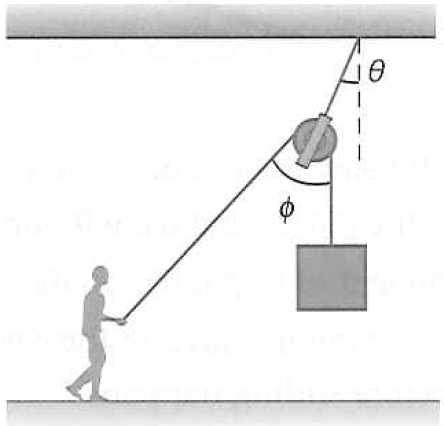
\includegraphics[width=.4\textwidth]{201d8637.png}
    \end{figure}
    \begin{parts}
        \part $\phi=60^{\circ}$,
        \begin{subparts}
            \subpart 求$\theta$。find $\theta$,\zh{2}
            \subpart 求纜繩的張力。find the tension in the cable.\zh{2}
        \end{subparts}
        \part 現在鮑勃試著更用力地拉繩子,以使角度 $\theta$ 等於 $\phi$。這有可能嗎?請簡要解釋。\\Now Bob tries to pull the string harder to make the angle $\theta$ that equals $\phi$. Is it possible? Explain briefly. \zh{2}
    \end{parts}
    \dlines{1}
    \clearpage
    \dlines{1}
}{
    \par
    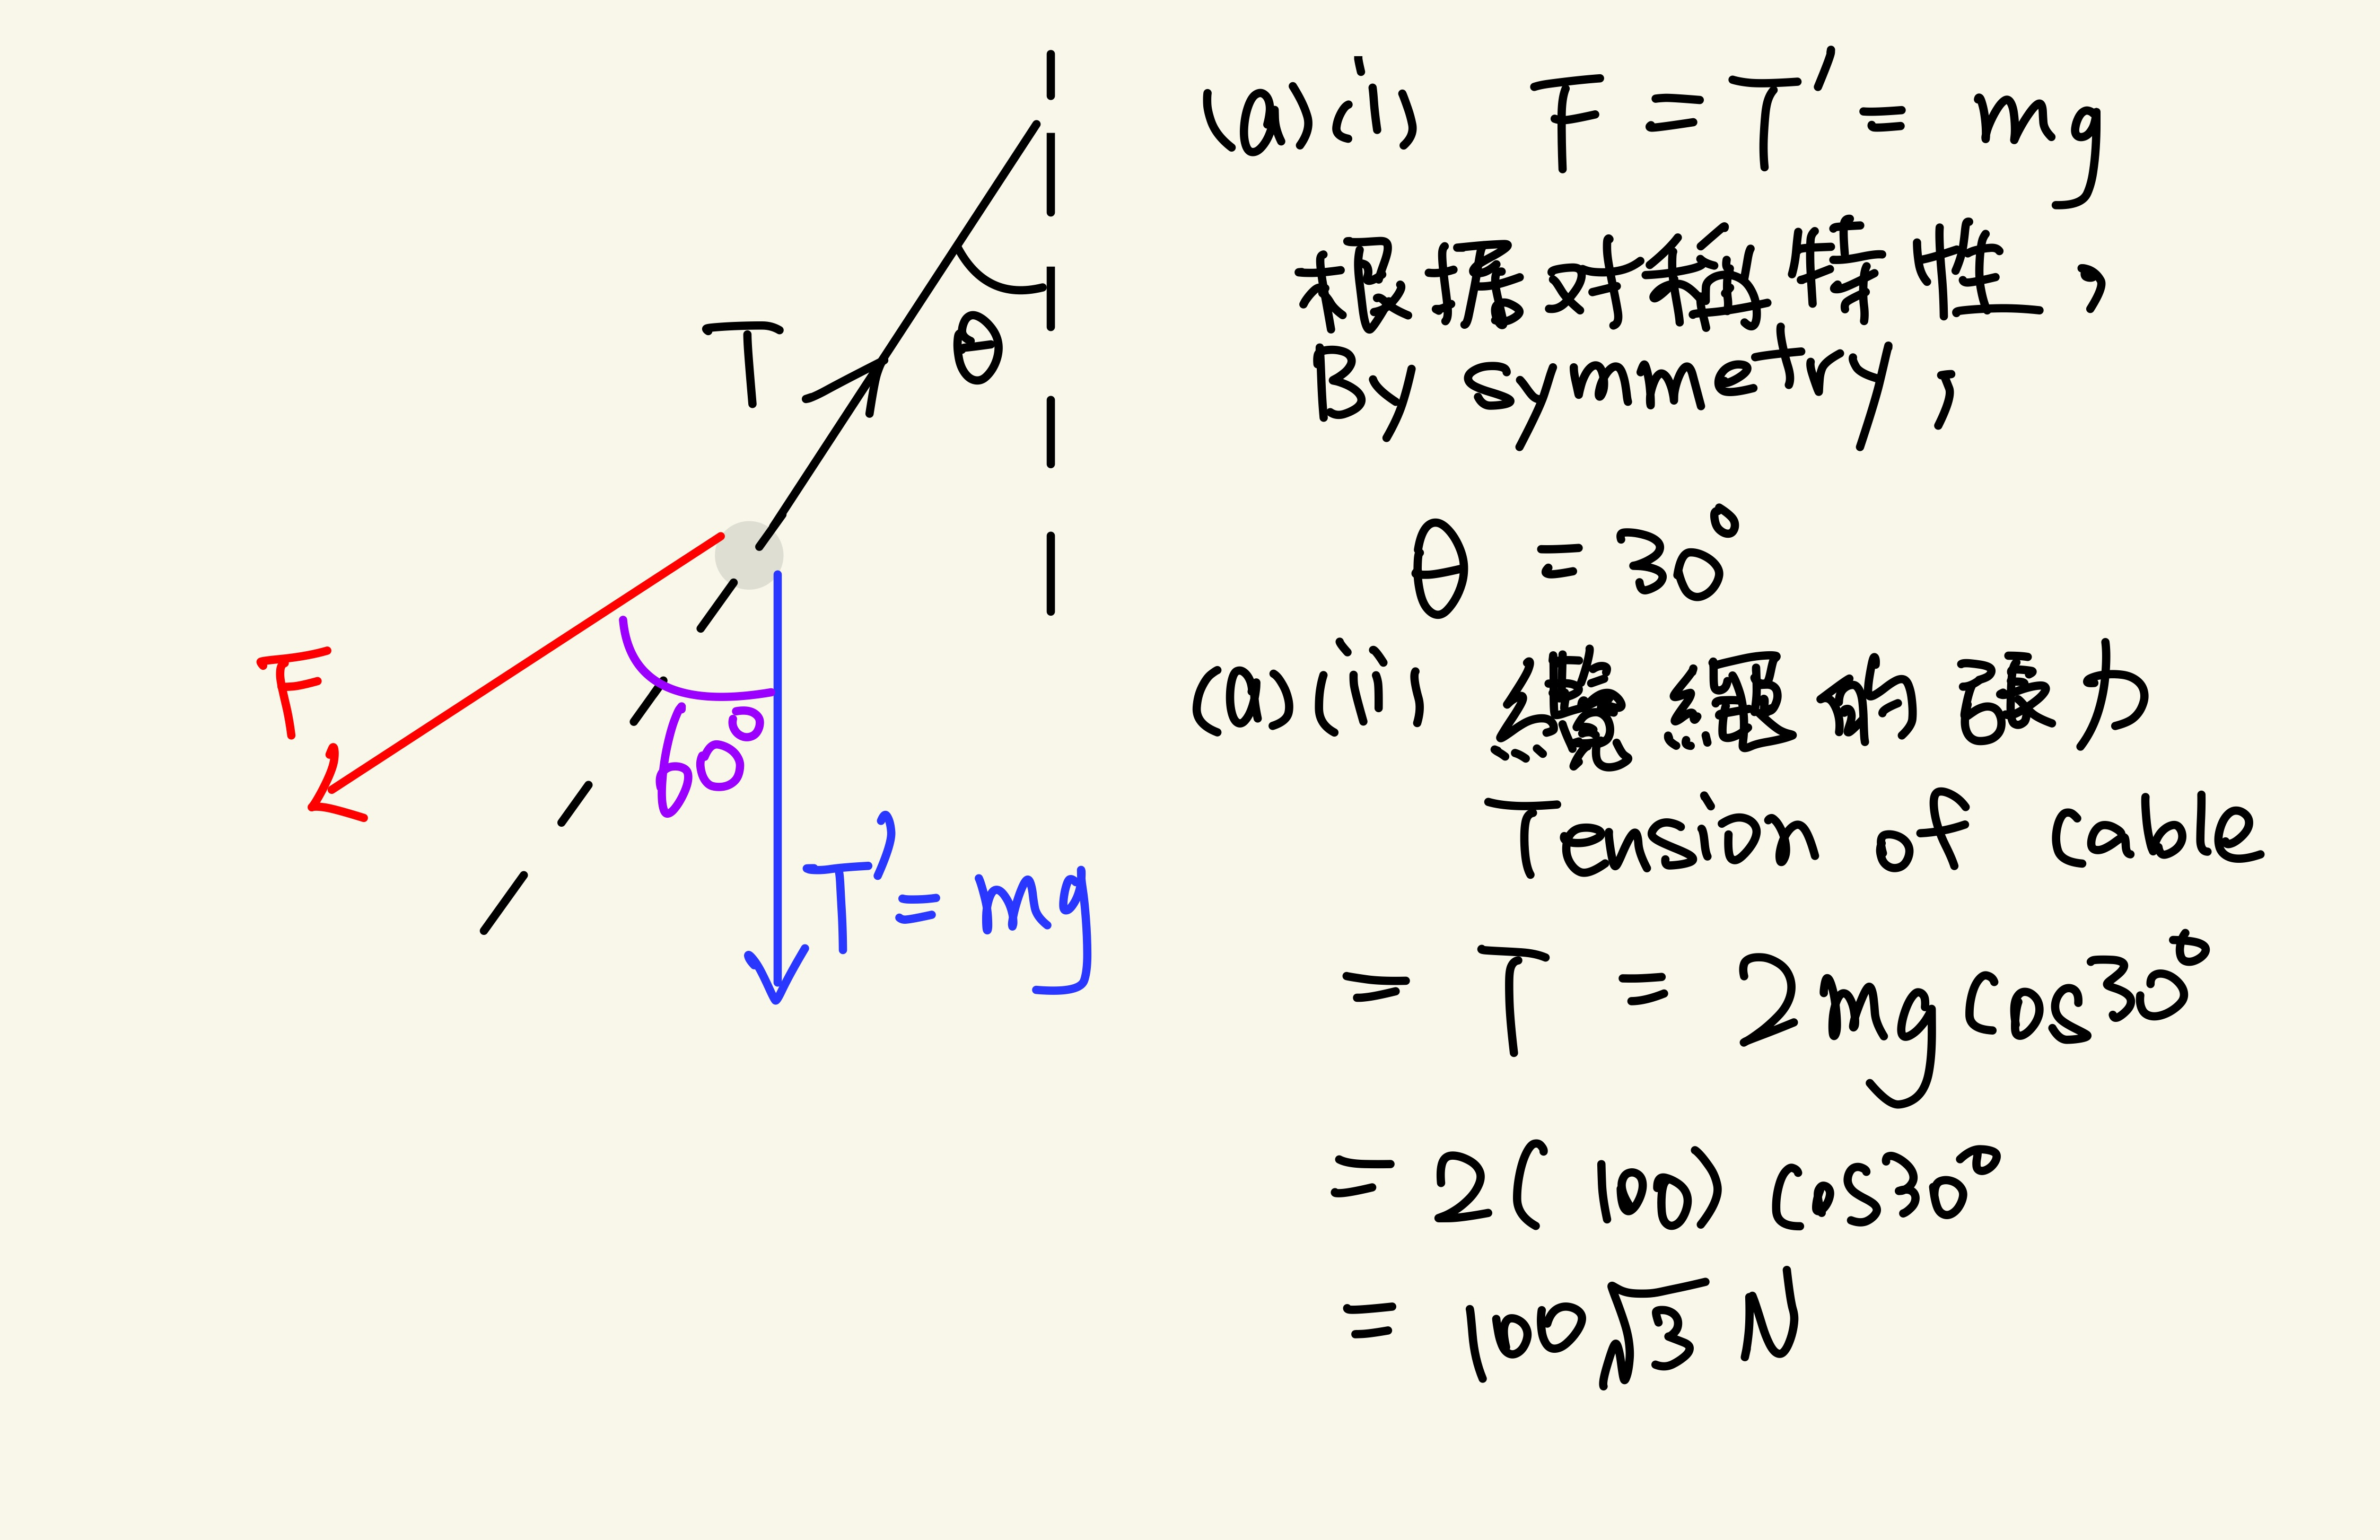
\includegraphics[width=.8\textwidth]{585f8ab0.png}
    \\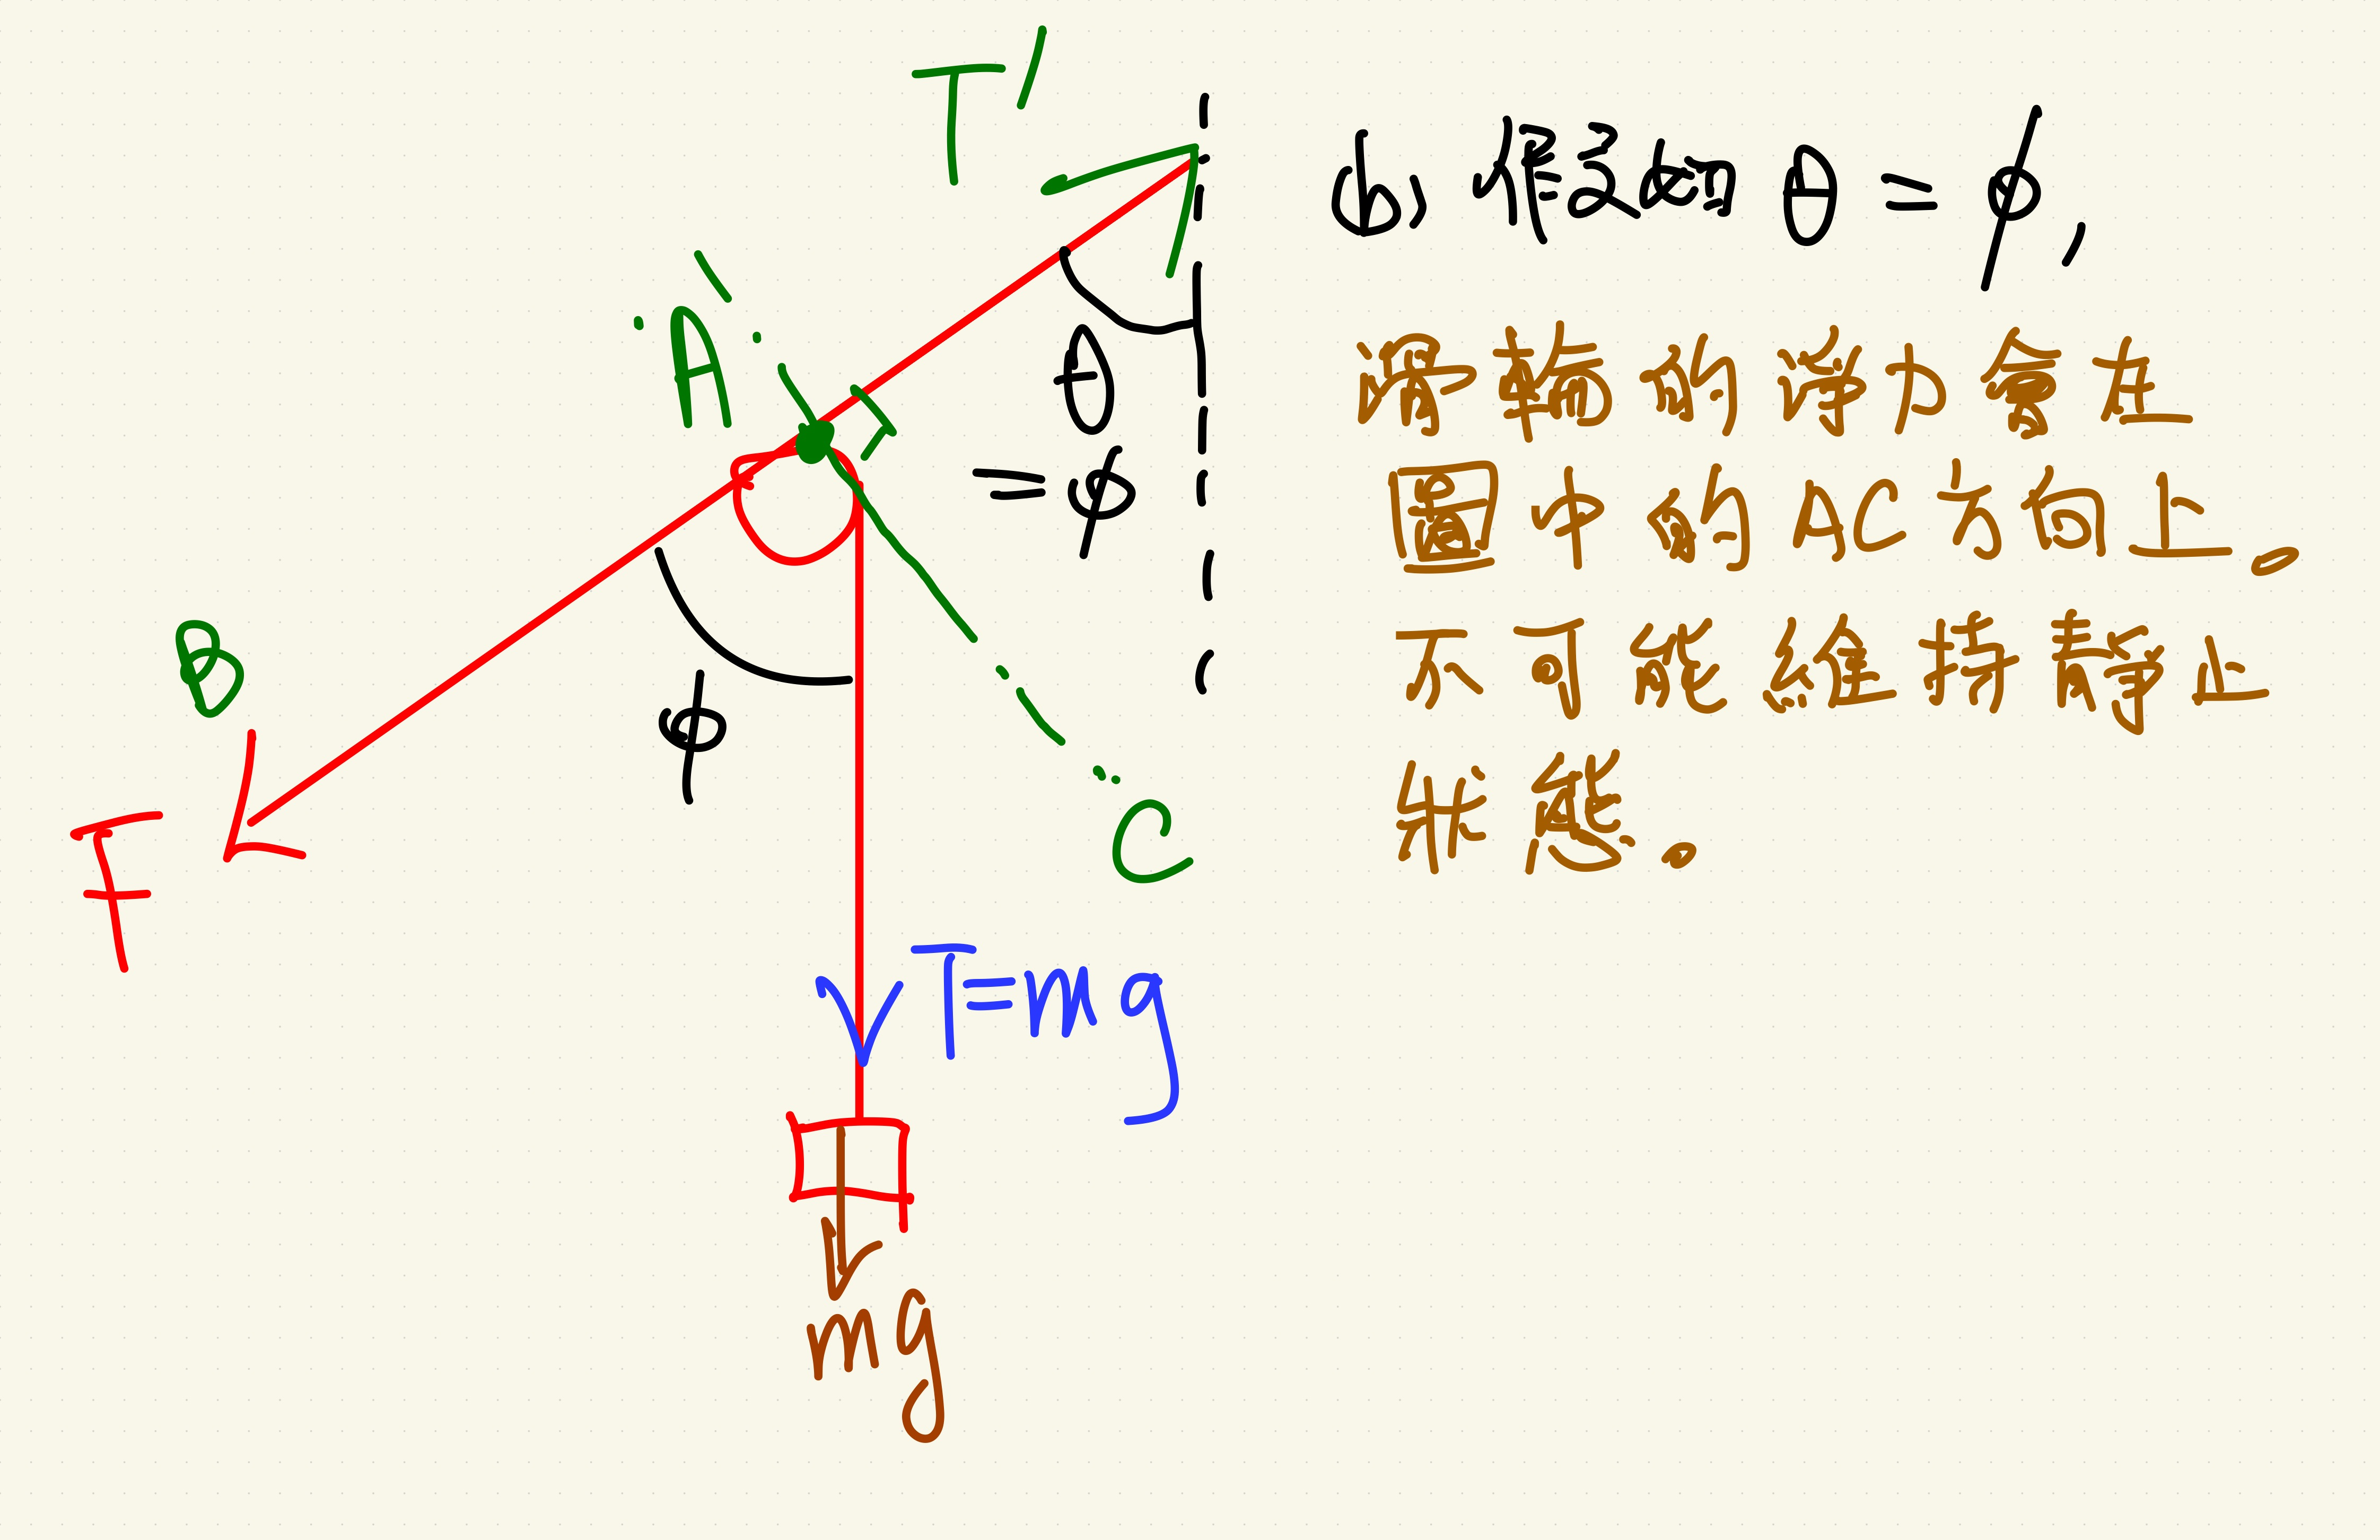
\includegraphics[width=.8\textwidth]{3ff7f052.png}
    \\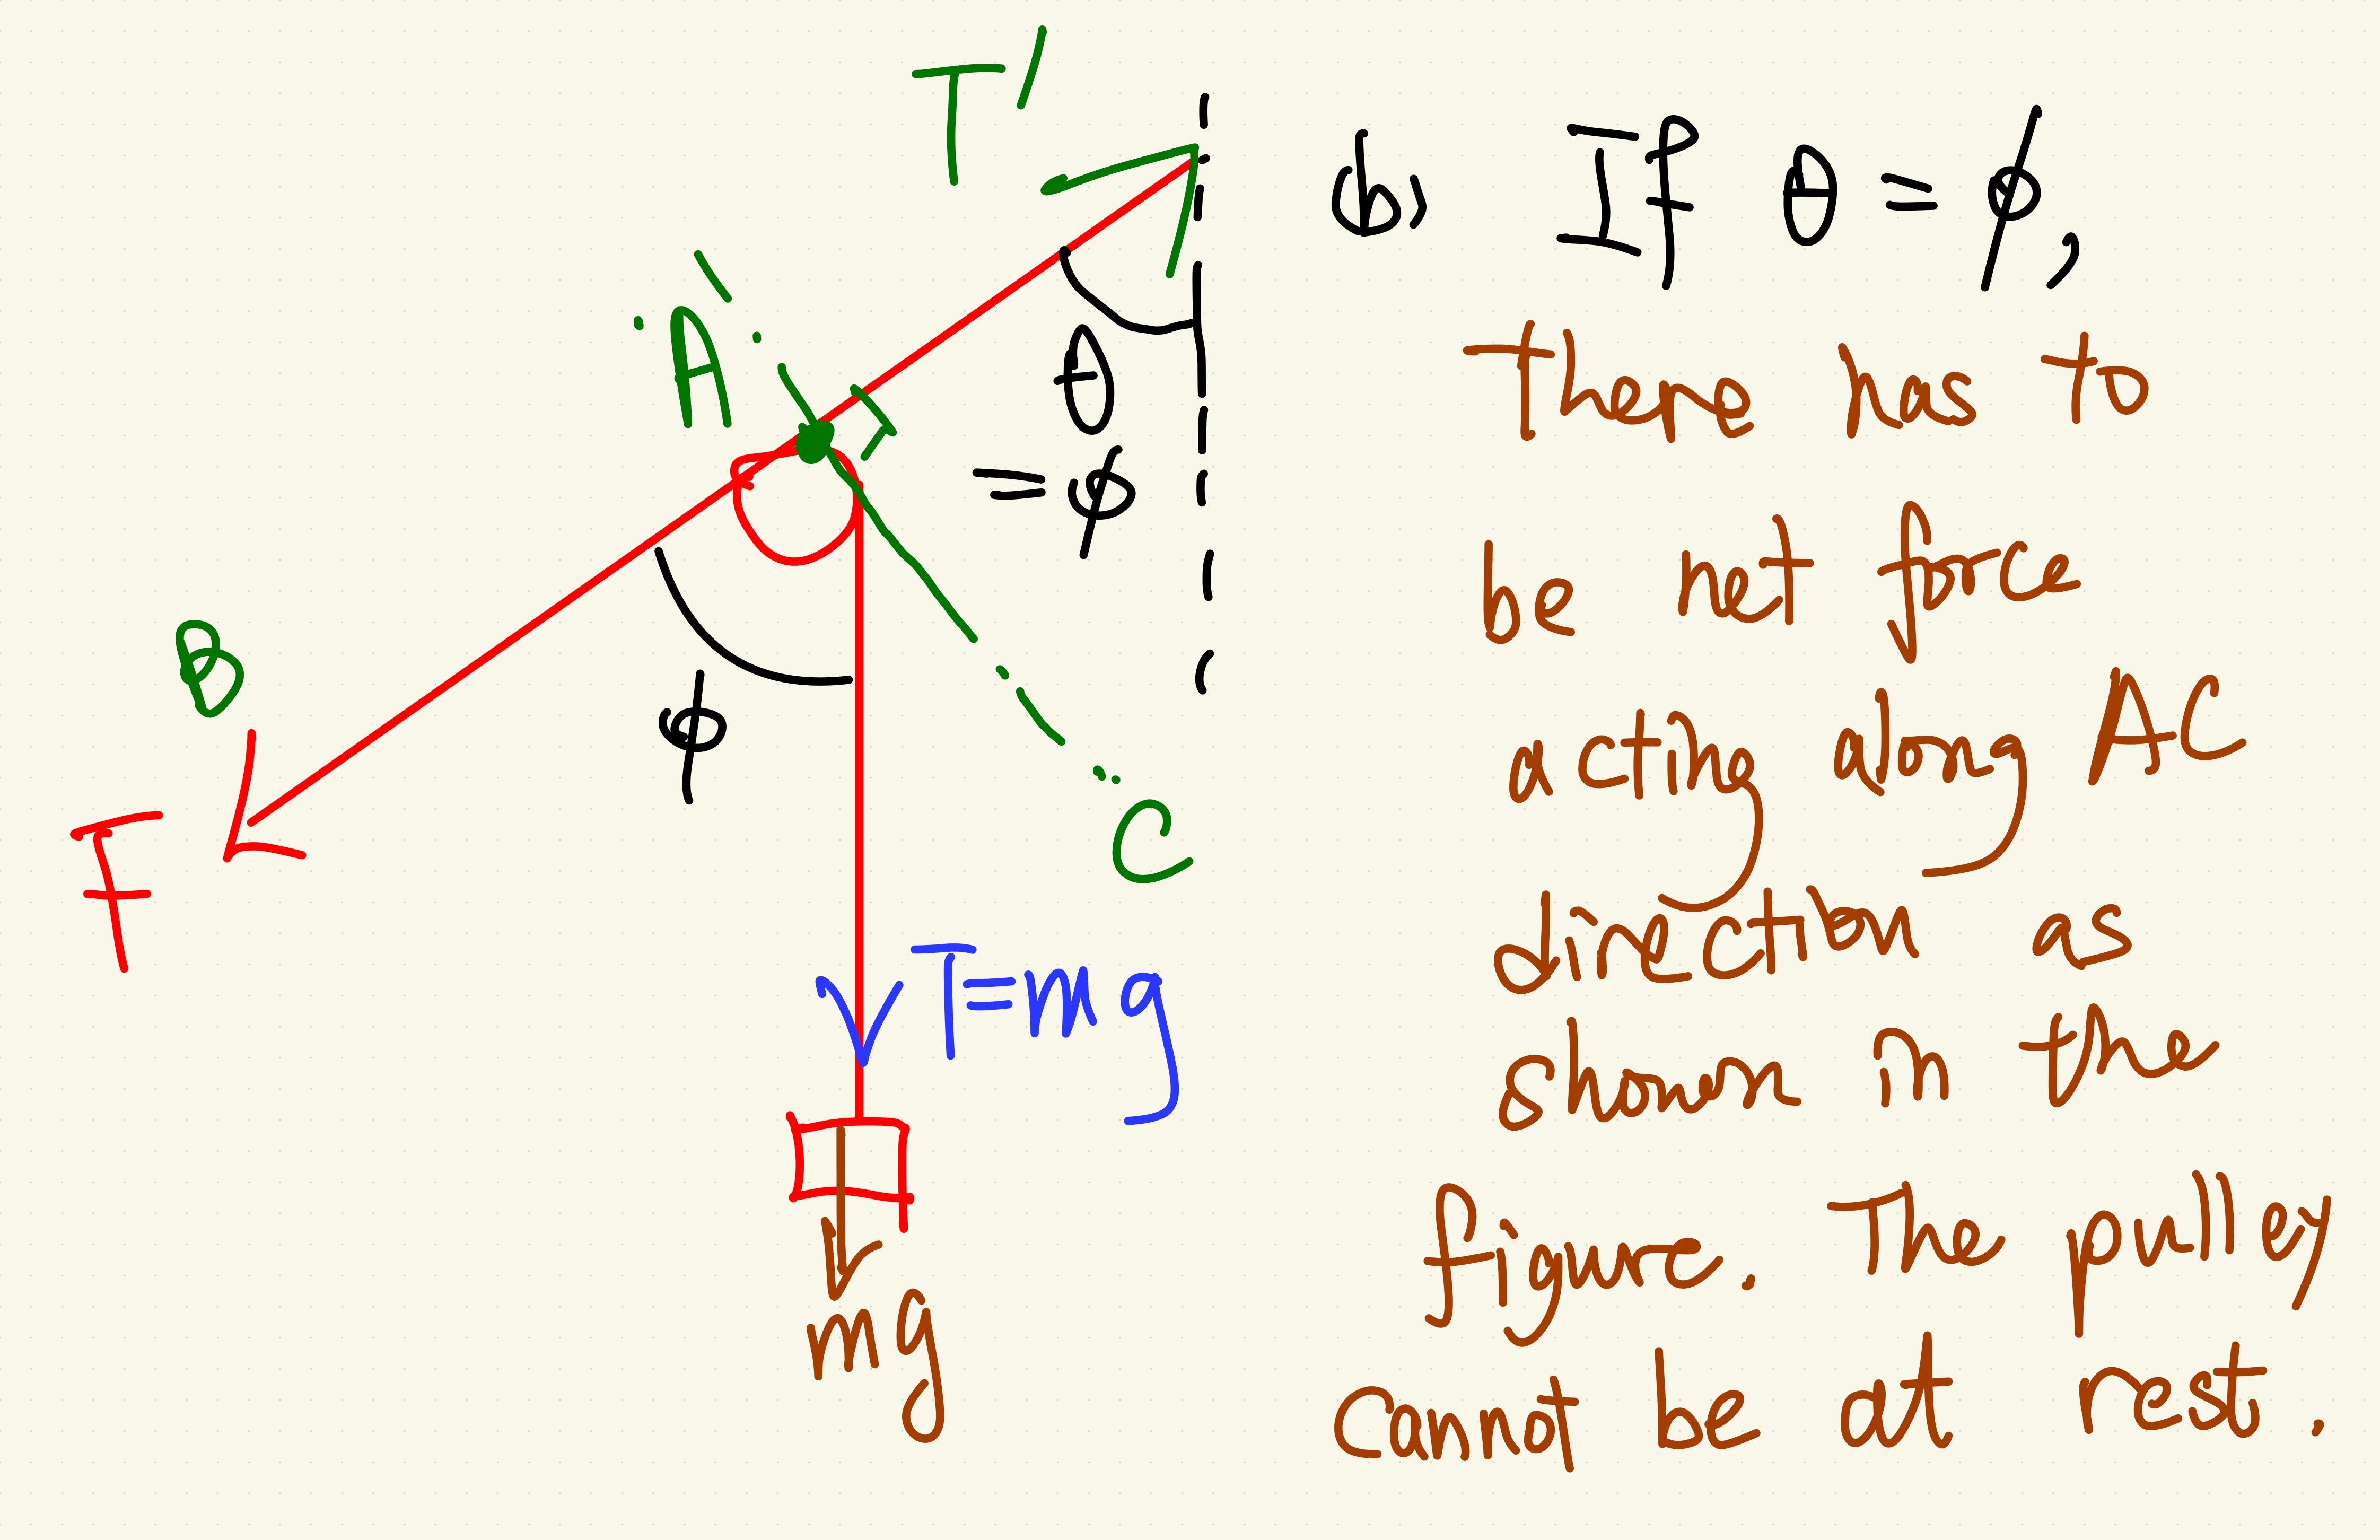
\includegraphics[width=.8\textwidth]{813bf005.png}
}


\newprob{lq2}{
    一本質量為0.5 kg 的書A放在一本質量為1 kg 的書B上方。兩本書都靜止在一個傾斜角度為$\theta$的斜面上,如圖所示。\\ A book A of mass 0.5 kg is placed on top of another book B of mass 1 kg. Both books are at rest on an inclined plane of inclination angle $\theta$ as shown.
    \bigskip
    \begin{figure}[h!]
        \centering
        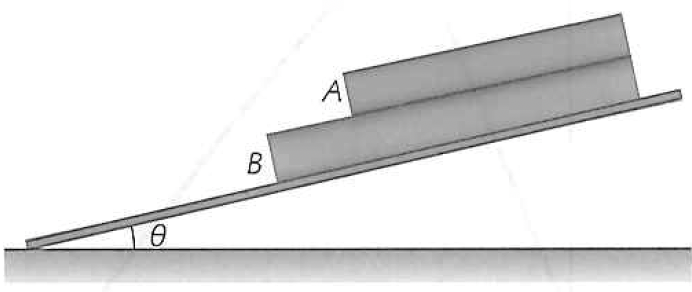
\includegraphics[width=.4\textwidth]{0dd56b85.png}
    \end{figure}
    \bigskip
    \begin{parts}
        \part 假設角度 $\theta$ 為 \dg{15}。求書 A 受到書 B 施加的法向力和摩擦力。\zh{2}\\Suppose the angle $\theta$ is \dg{15}. Find the normal reaction and friction exerted on A by B.
        \part 角度 $\theta$現在慢慢地增加。\\The angle $\theta$ increases gradually.
        \begin{subparts}
            \subpart 書本在角度 $\theta$ 達到 \dg{45}之前都保持靜止。求書 B 和斜面之間的最大摩擦力量值。\\ The books stay at rest until $\theta$ reaches \dg{45}. Find the magnitude of limiting friction between book B and the inclined plane. \zh{2}
            \subpart 書本在角度 $\theta$ 達到 \dg{60} 之前都保持連接在一起。使用(b)(i) 的答案,求書 A 和書 B 之間的最大摩擦力量值。\\The books stay attached to each other until $\theta$ reaches \dg{60}. Using (b)(i), find the limiting friction between books A and B. \zh{2}
        \end{subparts}

    \end{parts}
    \dlines{1}\clearpage\dlines{1}
}{
    \par
    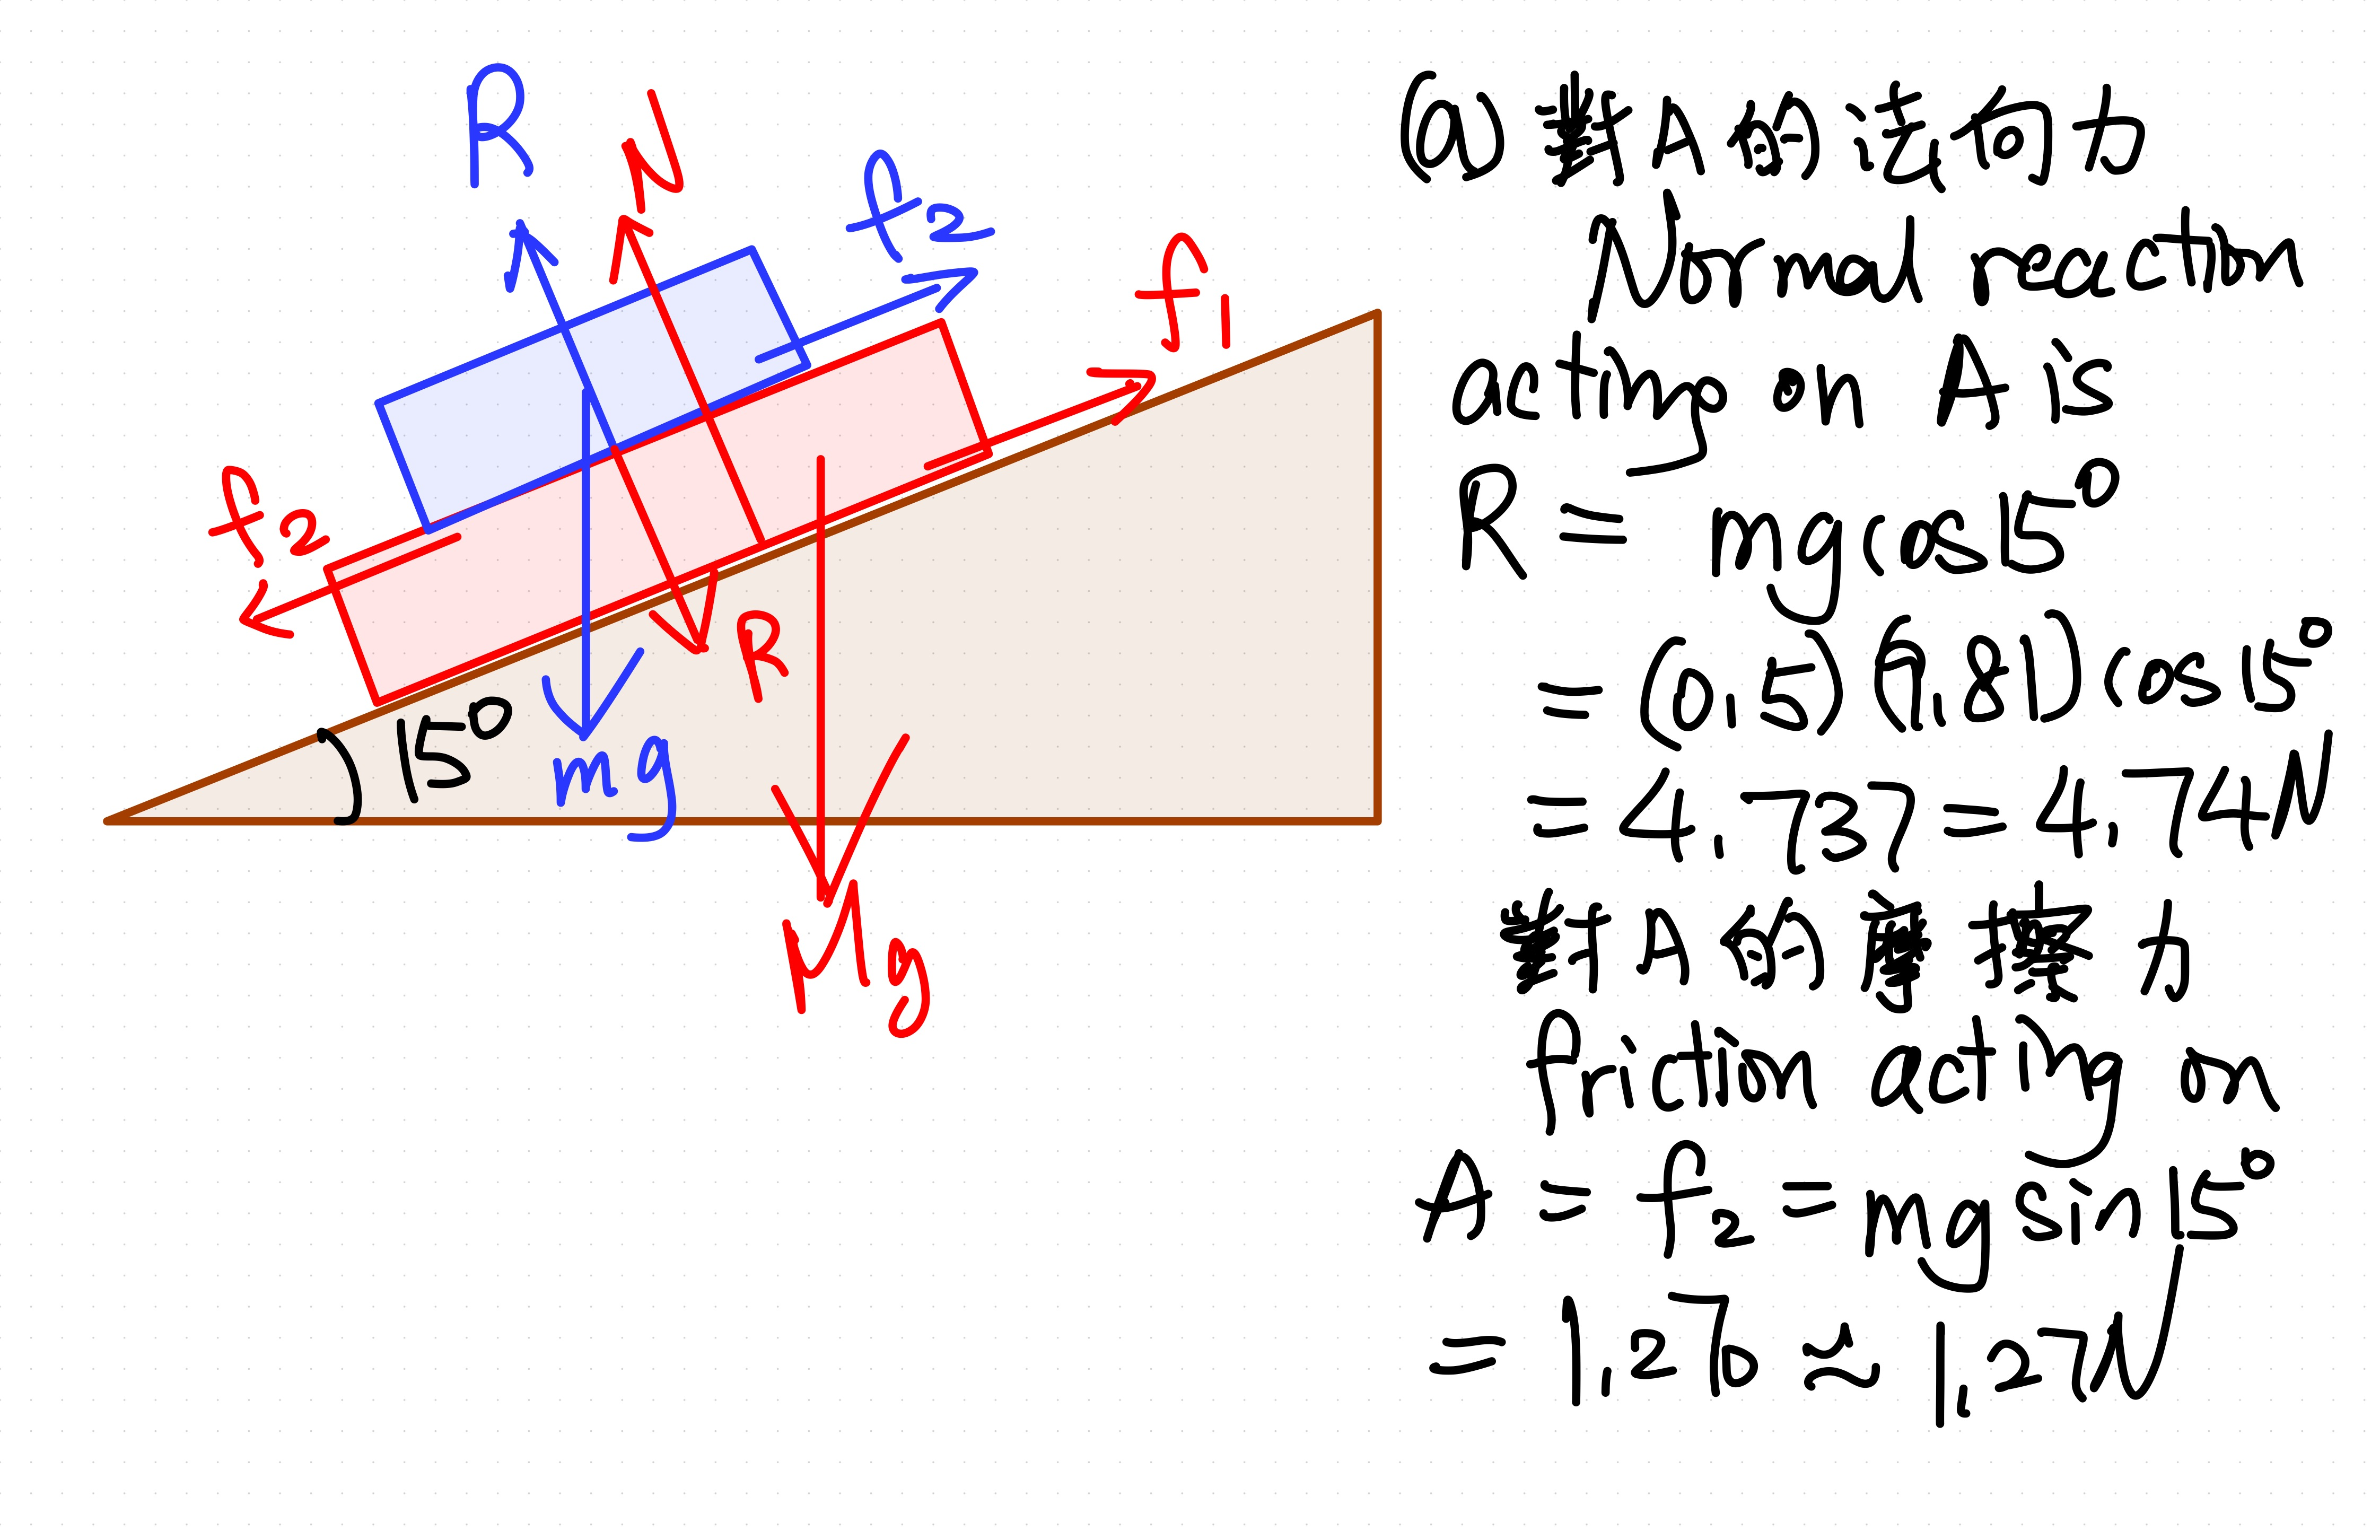
\includegraphics[width=.8\textwidth]{e519f0a6.png}\\
    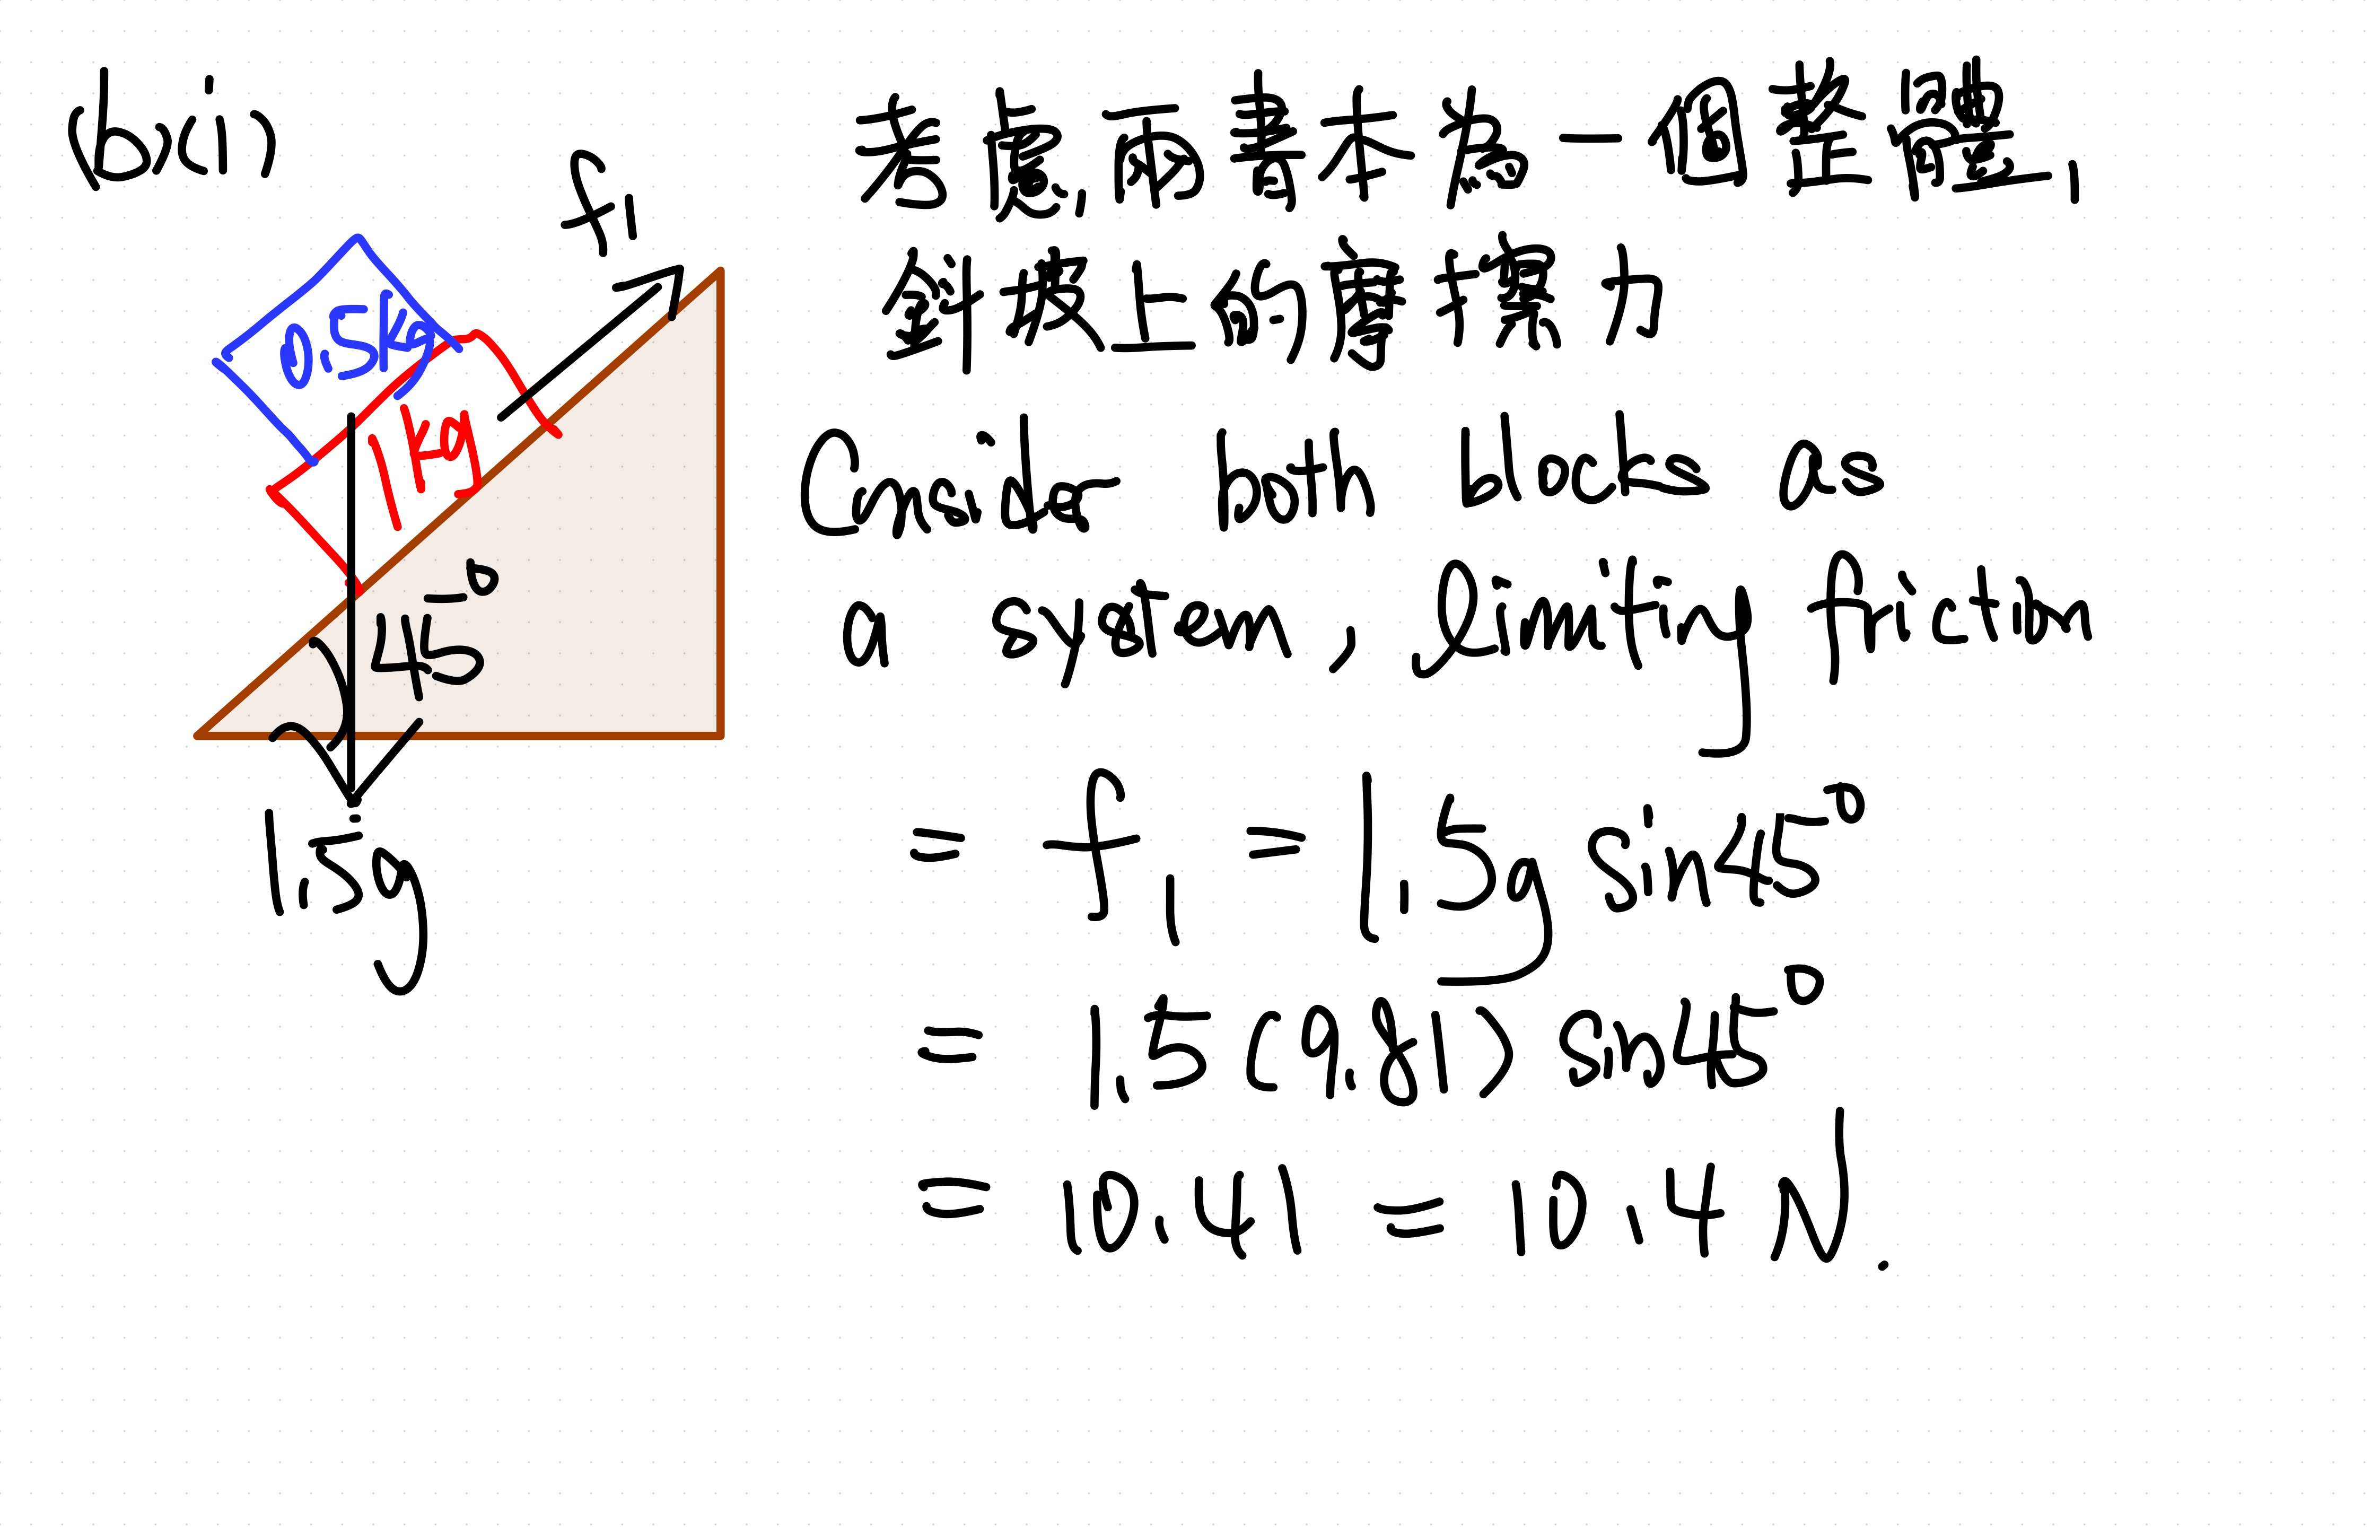
\includegraphics[width=.8\textwidth]{2331b9cf.png}\\
    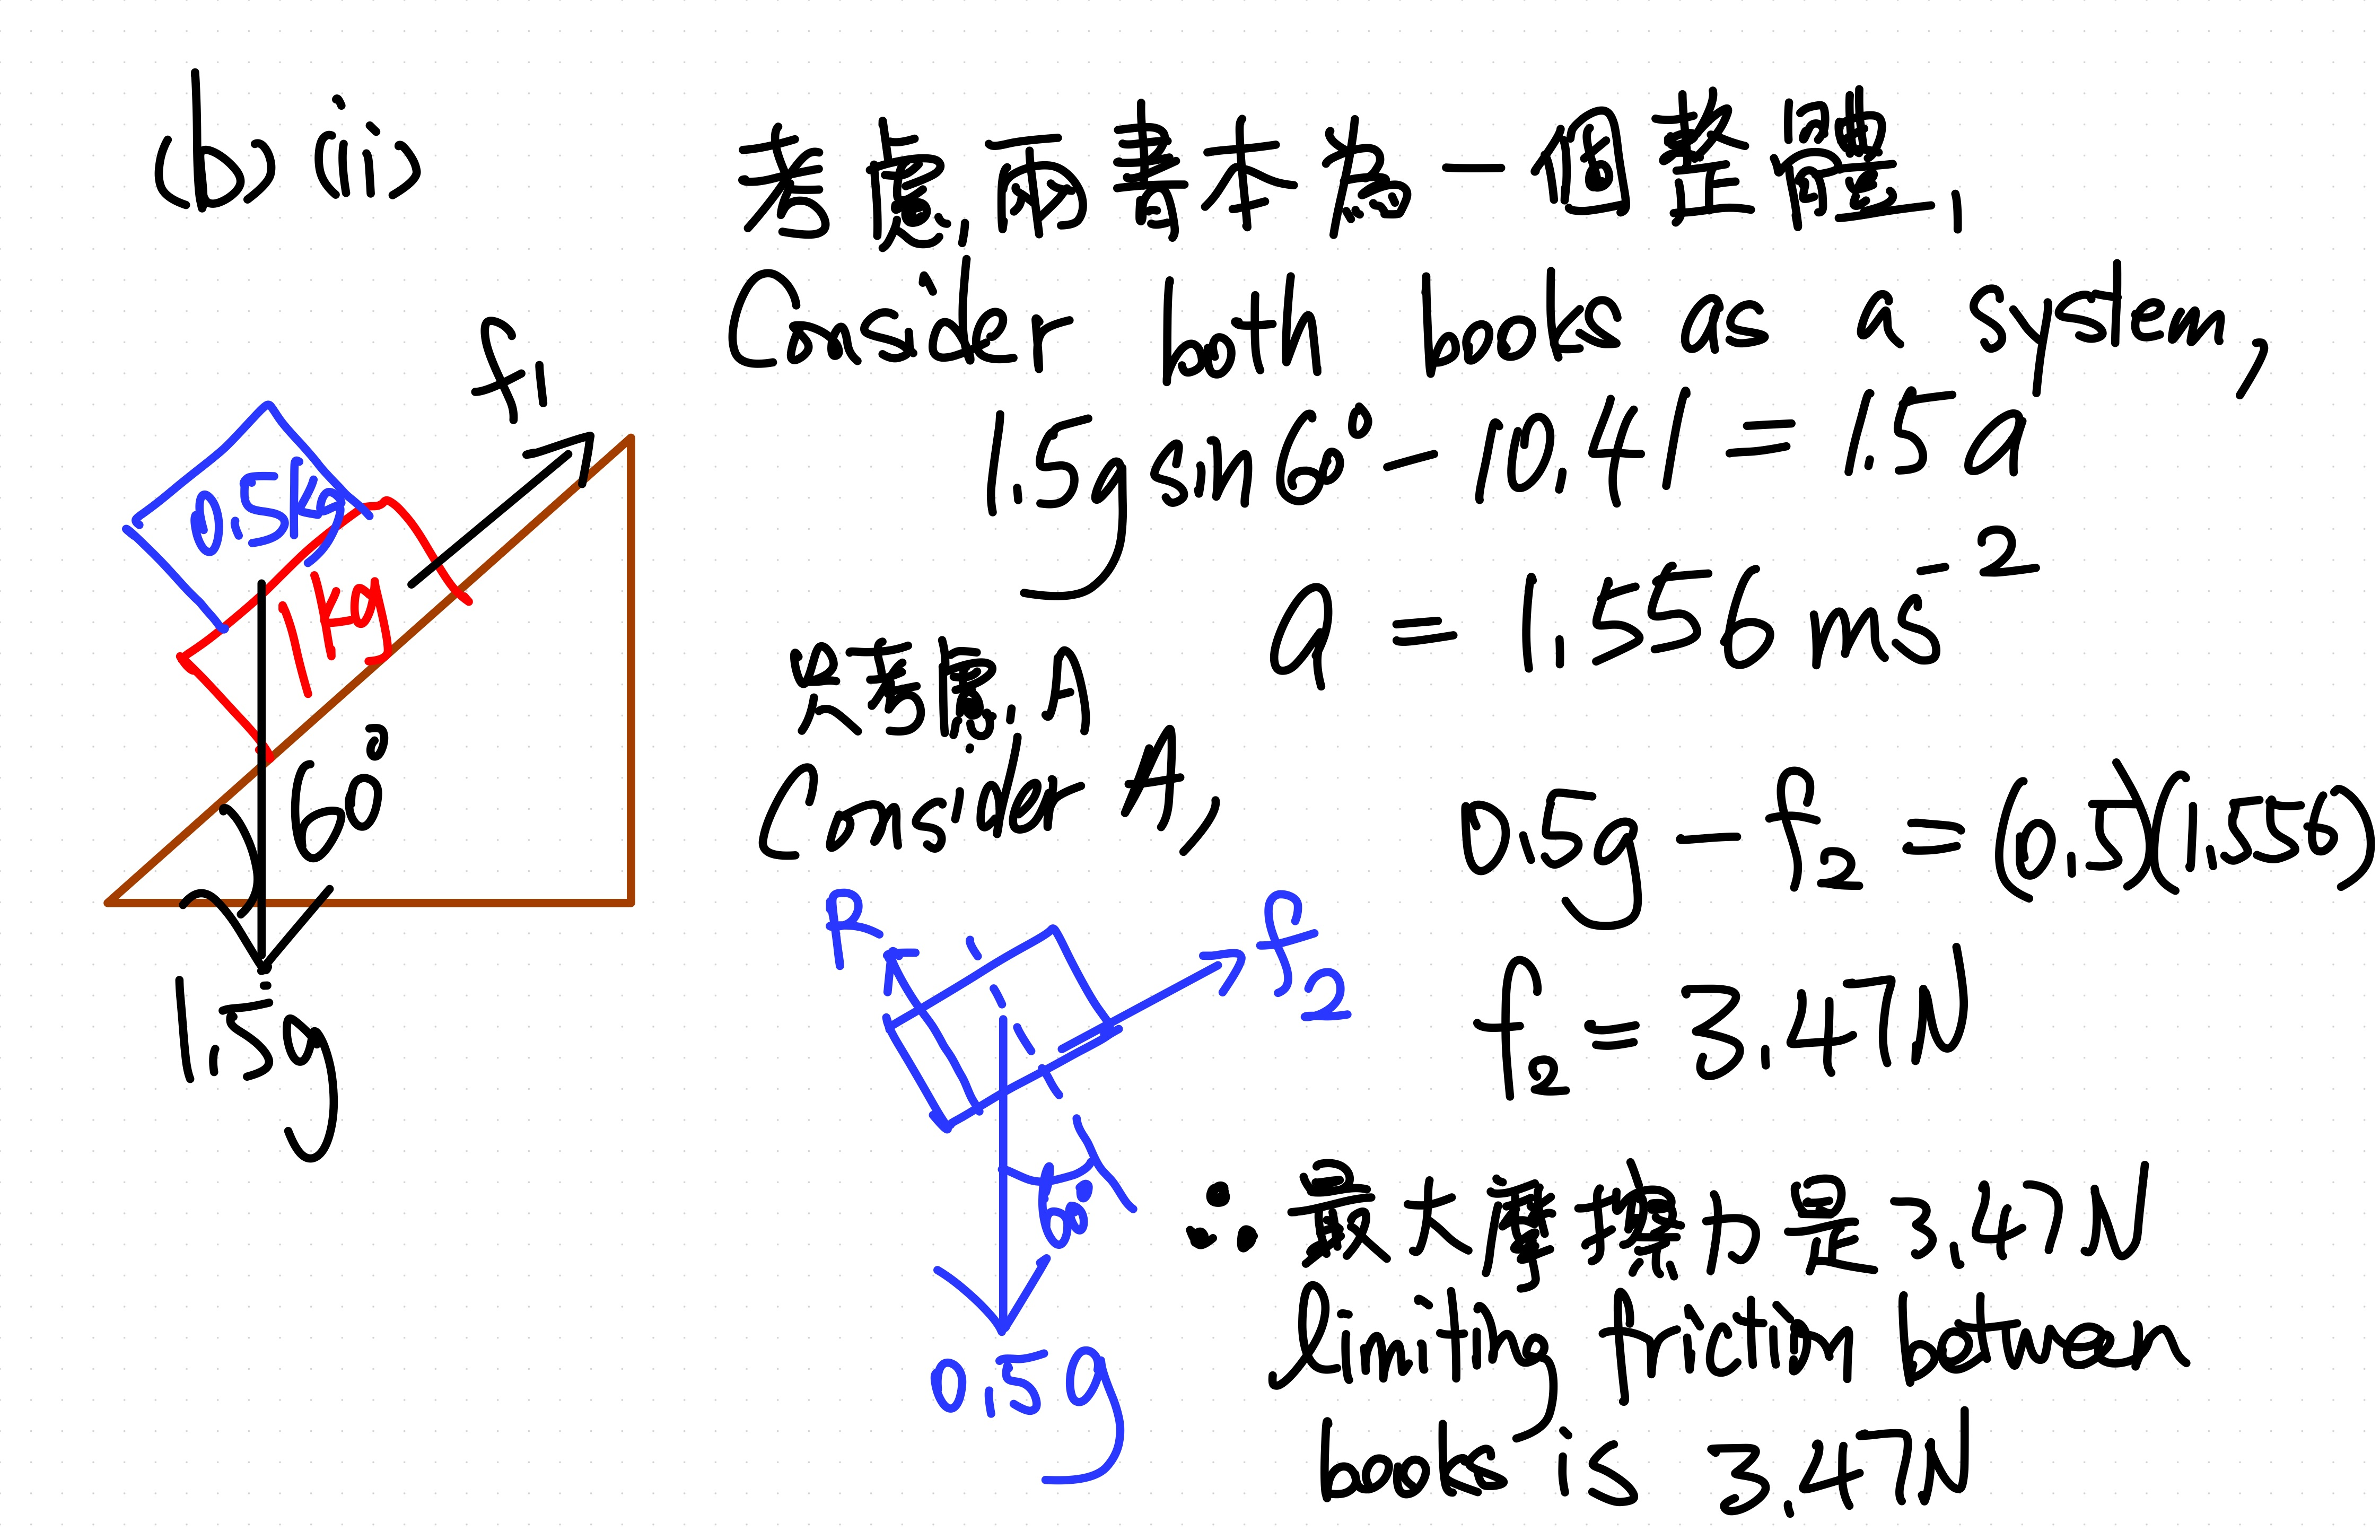
\includegraphics[width=.8\textwidth]{0fa0f589.png}
}

\newprob{lq3}{
    方塊X和Y的質量分別為4 kg和3kg,兩者以不能伸展的輕繩連接。一個25 N的恆力施於 Y使方塊以\vel{3.5}的恆速沿斜面上升,如上圖所示。斜面與水平成所成的角為$\theta$。每個方塊與斜面之間的摩擦力是2 N。
    \bigskip\par{\par\centering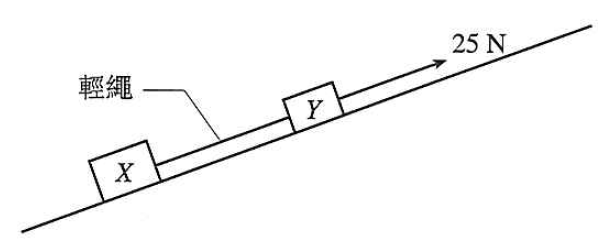
\includegraphics[width=.45\textwidth]{./img/ch2prob_2024-04-26-16-13-21.png}\par}\bigskip
    \begin{parts}
        \part 求角 $\theta$。\zh{3}
        \dlines{3}
        \clearpage
        \part 繩子突然在$t=\qty{4}{s}$斷裂。
        \begin{subparts}
            \subpart 描述方塊Y在$t=\qty{4}{s}$後的運動。\zh{1}
            \dlines{1}
            \subpart 證明方塊X在$t=\qty{5}{s}$的一瞬間靜止。\zh{2}
            \dlines{2}
            \subpart 完成以下對方塊 X 由 $t=\qty{0}{s}$至 $t=\qty{10}{s}$的速度-時間關係線圖。\zh{2}
            \bigskip\par{\par\centering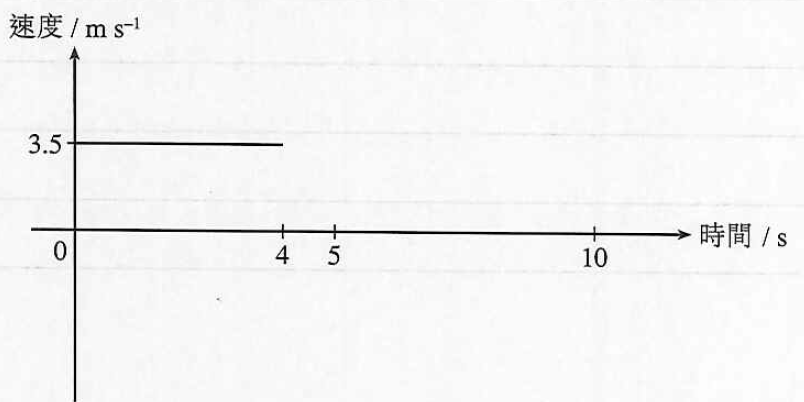
\includegraphics[width=.6\textwidth]{./img/ch2prob_2024-04-26-16-18-58.png}\par}\bigskip
        \end{subparts}
    \end{parts}
}{
    \par{\par\centering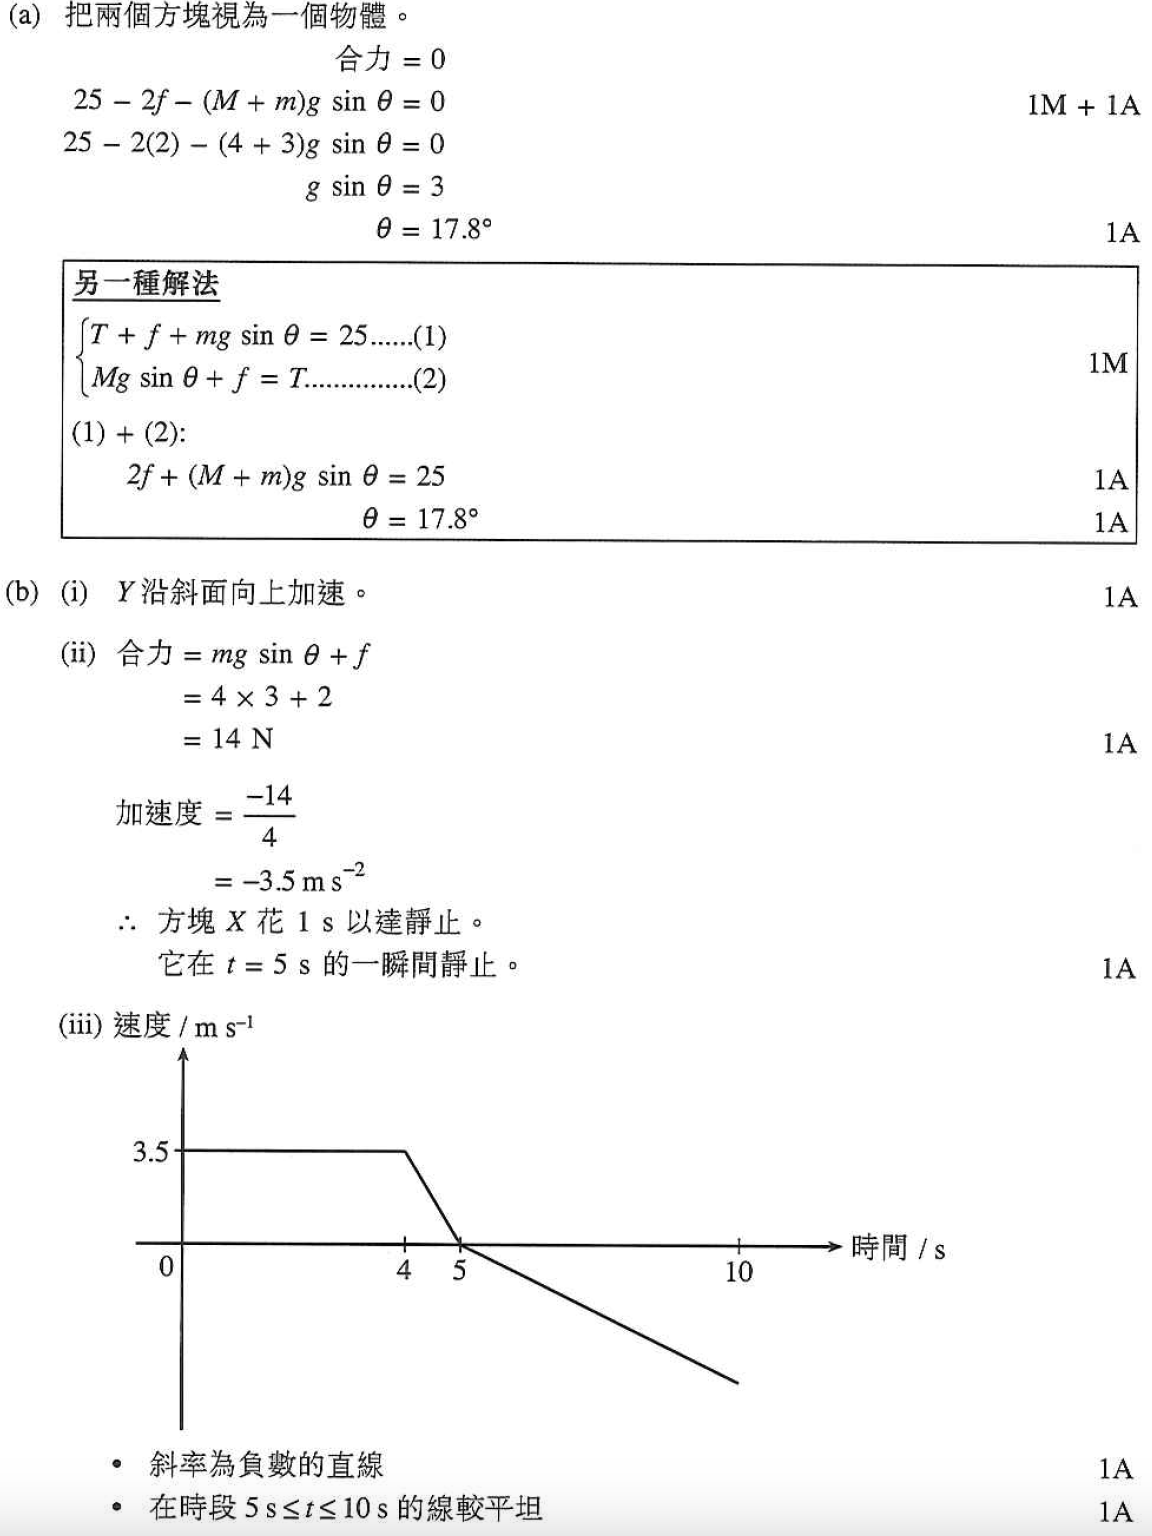
\includegraphics[width=\textwidth]{./img/ch2prob_2024-04-28-22-31-49.png}\par}
}

\newprob{lq4}{
    天花板上吊了一個輕質滑輪。有一根定長的細繩跨過滑輪,繩端各懸掛一件重物,如圖。
    \bigskip\par{\par\centering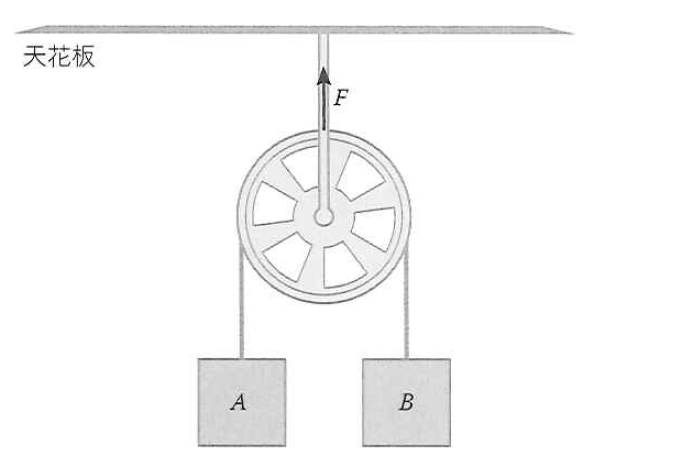
\includegraphics[width=.4\textwidth]{./img/ch2prob_2024-04-26-16-26-24.png}\par}\bigskip
    \begin{parts}
        \part 如果兩物的質量相同,各為5 kg,放手後, $F$的量值是多少? \zzh{2}
        \dlines{2}
        \part 如果$B$的質量改為2 kg,放手後,$F$的量值 是多少? \zzh{3}
        \dlines{3}
    \end{parts}
}{
    \par{\par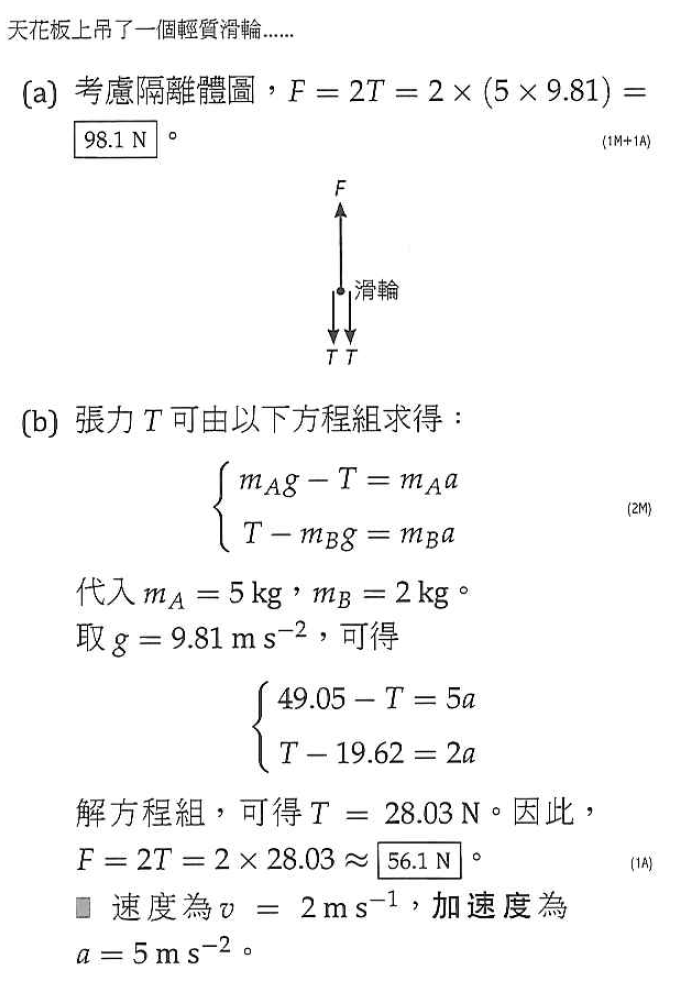
\includegraphics[width=.5\textwidth]{./img/ch2prob_2024-04-26-16-30-25.png}\par}
}

\newprob{lq5}{
    把質量5 kg的方塊放到斜台上。方塊從靜止開 始滑行,三秒後仍未離開斜台。
    \bigskip\par{\par\centering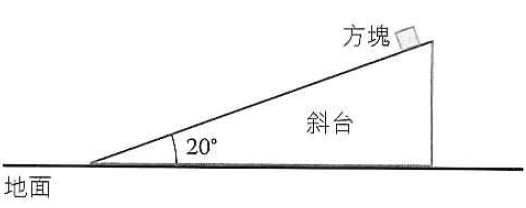
\includegraphics[width=.4\textwidth]{./img/ch2prob_2024-04-26-16-33-40.png}\par}\bigskip
    斜台的質量為方塊的10倍。略去摩擦力不計。
    \begin{parts}
        \part 如果斜台固定不動,求放手三秒後,方塊的 速率。 \zzh{2}
        \part 如果斜台非固定,可自由移動,那麼方塊的 加速度是否仍平行於斜台的斜面?試扼要解 釋。\zzh{2}
    \end{parts}
    \dlines{1}
}{
    \par{\par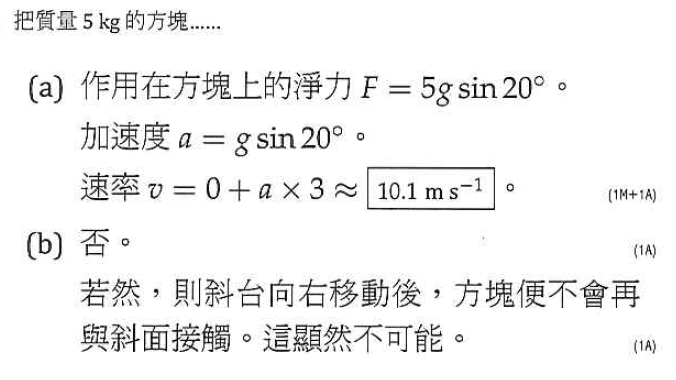
\includegraphics[width=.5\textwidth]{./img/ch2prob_2024-04-26-16-37-35.png}\par}
}


\newprob{mc1}{
    一個裝有機關的籐籃,以滑輪和細繩吊在天花板 上,如圖。細繩的一端繞在籐籃的捲輪上,捲 輪的旋轉速率可調整。\bigskip
    \par{\par\centering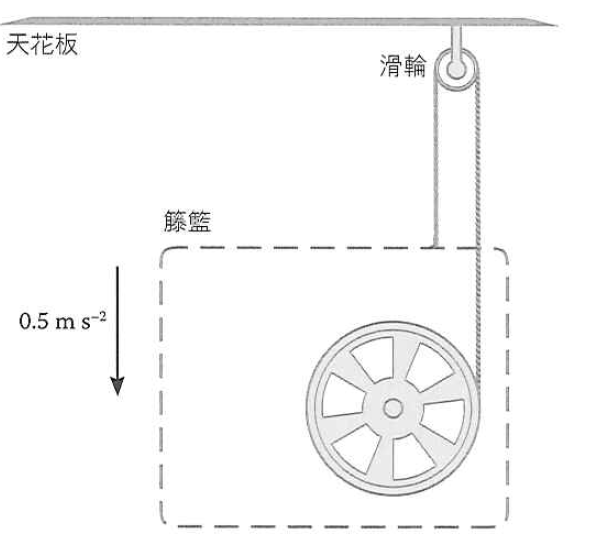
\includegraphics[width=.4\textwidth]{./img/ch2prob_2024-04-26-16-39-57.png}\par}\bigskip
    籐籃以\acc{0.5}匀減速下降。假設籐籃連機關 的總質量為10 kg。求細繩的張力。
    \begin{tasks}
        \task 44.1 N
        \task 46.6 N
        \task 47.8 N
        \task 49.1 N
    \end{tasks}

}{
    B
    \par{\par\centering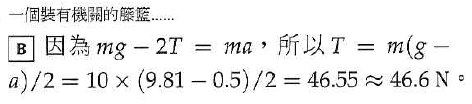
\includegraphics[width=.7\textwidth]{./img/ch2prob_2024-04-28-23-19-14.png}\par}
}

\newprob{mc2}{
    重物A 下以細繩吊着另一個重物B。細繩不可延 伸,且質量可略去不計。
    \par{\par\centering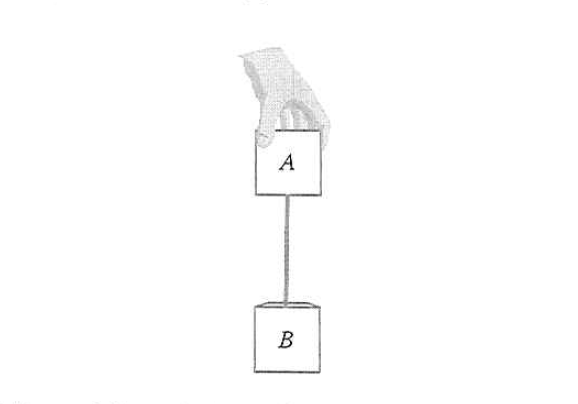
\includegraphics[width=.35\textwidth]{./img/ch2prob_2024-04-26-16-44-52.png}\par}
    放手一段時間後,重物B的加速度是多少?
    \begin{tasks}
        \task 大於$g$
        \task 小於$g$
        \task 等於$g$
        \task  由重物 B 的質量決定
    \end{tasks}
}{C
    \par{\par\centering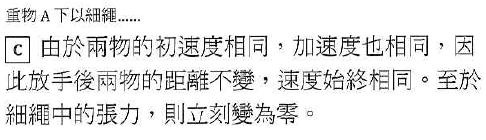
\includegraphics[width=.7\textwidth]{./img/ch2prob_2024-04-28-23-17-00.png}\par}}

\newprob{mc3}{
    重物A下以彈簧吊着另一個重物B。彈簧由於B 的重量而拉長了。
    \par{\par\centering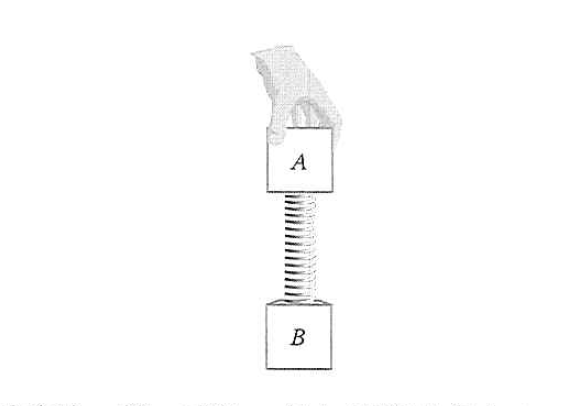
\includegraphics[width=.35\textwidth]{./img/ch2prob_2024-04-26-16-42-41.png}\par}
    放手後的一刻,重物B的加速度是多少?
    \begin{tasks}
        \task 大於$g$
        \task 小於$g$
        \task 等於$g$
        \task  由重物 B 的質量決定
    \end{tasks}
}{B
    \par{\par\centering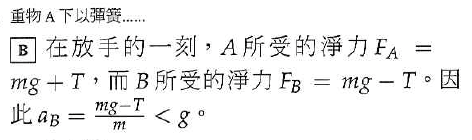
\includegraphics[width=.7\textwidth]{./img/ch2prob_2024-04-28-23-17-21.png}\par}}

\newprob{mc4}{
    從飛機投下一個密封的木箱,木箱內有一個電子 磅,磅上放了一個2 kg的砝碼。
    \par{\par\centering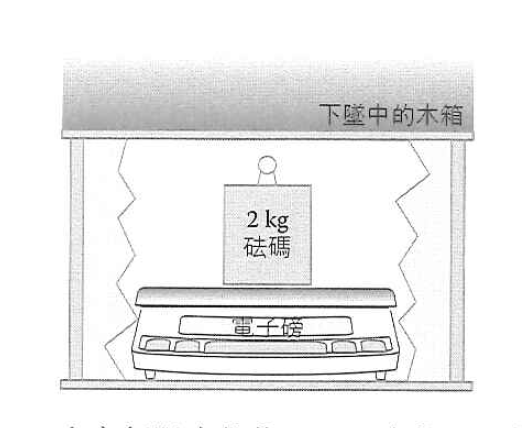
\includegraphics[width=.35\textwidth]{./img/ch2prob_2024-04-26-16-46-05.png}\par}
    在空氣阻力的作用下,木箱現以終端速度下墜。 如果木箱保持正立,磅的讀數R是多少?
    \begin{tasks}
        \task $R=\left( 2\times 9.81 \right)$ N
        \task $0<R<\left( 2\times 9.81 \right)$ N
        \task $R=0$ N
        \task 視下墜的速率而定
    \end{tasks}

}{A
    \par{\par\centering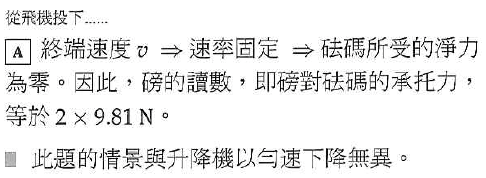
\includegraphics[width=.7\textwidth]{./img/ch2prob_2024-04-28-23-16-28.png}\par}}

\newprob{mc5}{
    有一缸水在水平地面上滑行。下圖顯示那缸水在 兩段時間內的情況。
    \par{\par\centering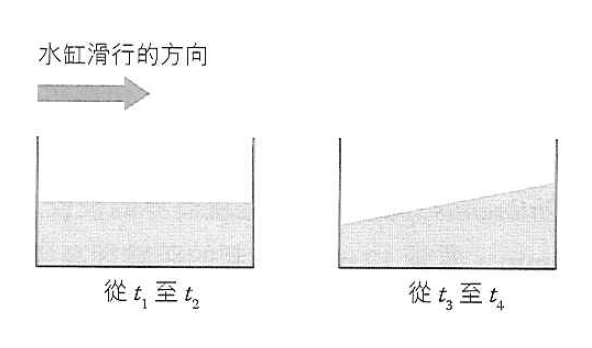
\includegraphics[width=.5\textwidth]{./img/ch2prob_2024-04-26-16-48-31.png}\par}
    有關那缸水的運動,下列哪項必定正確?
    \begin{statements}
        \task 從 $t_1$至 $t_2$,那缸水靜止。
        \task 從 $t_3$至$t_4$,那缸水所受的力較大。
        \task 從 $t_3$至$t_4$,那缸水在減速。
    \end{statements}
    \begin{tasks}
        \task 只有(1) \tab\tab (1) only
        \task 只有(2) \tab\tab (2) only
        \task 只有(1)和(3) \tab\tab (1) and (3) only
        \task 只有(2)和(3) \tab\tab (2) and (3) only
    \end{tasks}

}{D
    \par{\par\centering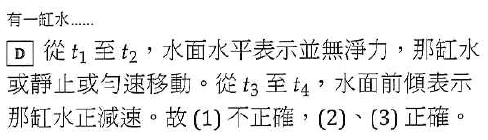
\includegraphics[width=.7\textwidth]{./img/ch2prob_2024-04-28-23-15-45.png}\par}}

